\documentclass[11pt,a4paper]{article}
\usepackage{graphicx}
\usepackage{amsfonts,amsmath}
\usepackage{listings}
\usepackage[T1]{fontenc}
\usepackage{float}
\usepackage[spanish]{babel}
\usepackage{geometry}

\title{\textbf{Sistemas Operativos: Práctica 2}}
\author{
    Shaofan Xu \\
    \and 
    Javier Maria Santa
    }
\date{\today}


\begin{document}
\maketitle

\clearpage
\section{Introducción}
El objetivo de esta práctica es utilizar mecanismos de sincronización para simular una block chain. En este entornos diversos procesos se forman mineros
para competir por el premio, así utlizando señales y semáforos para comunicar entre los procesos.
\section{Requisitos cumplidos y no cumplidos}
\subsection{Requisitos cumplidos}
Se han implementado correctamente los siguientes objetivos principales de la práctica:
\begin{itemize}
    \item \textbf{Gestión de múltiples procesos Minero:} Se ha implementado un fichero compartida protegido por mutex
    donde los procesos registran pid al entrar al sistema y eliminan al salir del sistema cuando llegan su tiempo límite, 
    así destruyendo el fichero el último proceso que sale.
    \item \textbf{Proceso de minería:} el primer proceso establece un objetivo inicial (0 en nuestro caso), y lanza señal para
    iniciar la ronda, posteriormente el primer minero que se encuentra el resultado escribe su resultado en \texttt{target.tgt}
    y lanzando otra señal para empezar la votación.
    \item \textbf{Sistema de votación:} una vez empezado el proceso de votación los procesos participantes deben comprobar el resultado del minero 
    candidato para votar si esta a favor o en contra, en cuyo caso, el proceso candidato irá comprobando los votos teniendo un máximo número de intento
    hasta tener más de un 50\% de voto a favor. Una vez tenido el resultado, el proceso candidato convierte en ganador, guardando su resultado en un
    fichero cuyo nombre es su pid, y el target de la siguiente ronda en \texttt{target.tgt}
    \item \textbf{Protección de zona crítica:} Para que el sistema no falle por problemas de concurrencia ni pierda señales por el camino, 
    hemos protegido las zonas críticas del código de cuatro formas:
    \begin{itemize}
    \item \textbf{Bloqueo inicial de señales:} Antes de entrar al bucle principal, se crea una máscara con \texttt{SIGUSR1}, \texttt{SIGUSR2} y \texttt{SIGALRM} 
    y usando sigprocmask. Así nos aseguramos de que, si llega una señal justo cuando esta leyendo o escribiendo en un fichero compartido,
     esta se quede pendiente y no rompe la ejecución a medias.
    \item \textbf{Control de interrupciones (EINTR):} Al mezclar semáforos y señales, pasaba que a veces la llamada a \texttt{sem\_wait()} se interrumpía por la llegada de una 
    señal antes de haber conseguido el semáforo. Para evitar que el código siga adelante asumiendo que tiene el recurso (lo que corrompería todo),protegemos las peticiones en un bucle: 
    \texttt{while (sem\_wait(...) == -1 \&\& errno == EINTR);}.
    Así, si una señal despierta al proceso por error, este vuelve a intentar.
    \item \textbf{Espera pasiva con sigsuspend:} Para cumplir con el enunciado y no freír la CPU con esperas activas, cuando el minero no está minando, 
    ni votando, ni gestionando la victoria, se pone a dormir llamando a \texttt{ sigsuspend(\&mask\_empty) }. Esto vacía la máscara de bloqueos temporalmente
     y deja al proceso suspendido hasta que llega una señal que lo despierta para la siguiente fase.
    \item \textbf{Evitar deadlocks en los hilos:} Durante las pruebas a menudo sucude que un proceso estaba bloqueado en el \texttt{pthread\_join} esperando a sus hilos y otro minero ganaba la ronda,
     el proceso bloqueado no podía recibir la señal \texttt{SIGUSR2} para ir a votar (se quedaba colgado).
    Como solución propuesta se desbloquea las señales con \texttt{SIG\_UNBLOCK} justo antes del join y volviéndolas a bloquear después. De 
    esta forma, la orden de votación entra sin problemas, los hilos abortan su ejecución y el programa no se atasca.
    \end{itemize}
\end{itemize}

\subsection{Requisitos no cumplidos}
Todos los requisitos obligatorios especificados en el enunciado han sido implementados 
y funcionan correctamente.

\section{Pruebas: Funcionamiento y Rendimiento}
\subsection{Entorno de ejecución}
Las pruebas y mediciones se han llevado a cabo bajo las siguientes condiciones de
hardware y software para garantizar la consistencia de los resultados:
\begin{itemize}
    \item Sistema Operativo: WSL2 (Ubuntu) sobre Windows 11.
    \item Hardware: 16 GB de memoria RAM.
    \item Herramienta de medición: Comando time de la shell de Linux.
\end{itemize}
\clearpage
\subsection{Pruebas de Funcionamiento}
Se han ejecutado diversas pruebas para asegurar el correcto funcionamiento del programa.

\subsubsection{Casos normales}
Se ejecutó el programa con parámetros correspondientes:
\begin{lstlisting}[language=bash]
./miner 3 8 & ./miner 5 8 & ./miner 10 8 & ./miner 10 1
\end{lstlisting}
El programa generó correctamente los archivo \texttt{.log} con la estructura especificada (Id, ronda, target, solución, etc), y la validación (accepted/rejected). Así imprimiendo en la terminal exactamente los mensajes requeridos:
\begin{figure}[H]
    \centering
    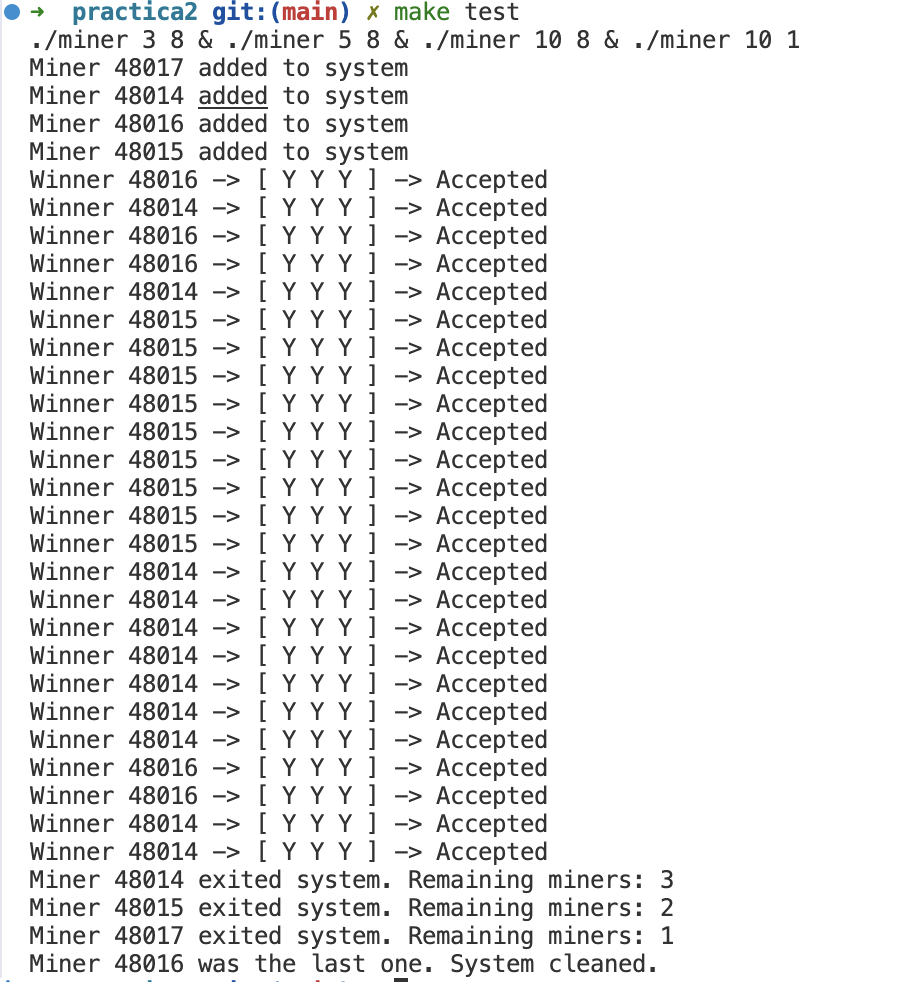
\includegraphics[width=0.8\textwidth]{image0.png}
    \caption{Ejecución de programa demostrando el proceso de entrada de los procesos mineros, los procesos minando, y destrucción del fichero cuando termina el último proceso }
\end{figure}

\subsubsection{Casos de errores}
Se probaron situaciones anómalas como:
\begin{itemize}
    \item \textbf{Falta de argumentos:} Al ejecutar \texttt{./miner} sin parámetros, el programa detecta el error, muestra el uso correcto \textit{``Usage ./miner < N\_SECS > < N\_THREADS >''}.
\end{itemize}

\subsection{Pruebas adicionales}
\begin{figure}[H]
    \centering
    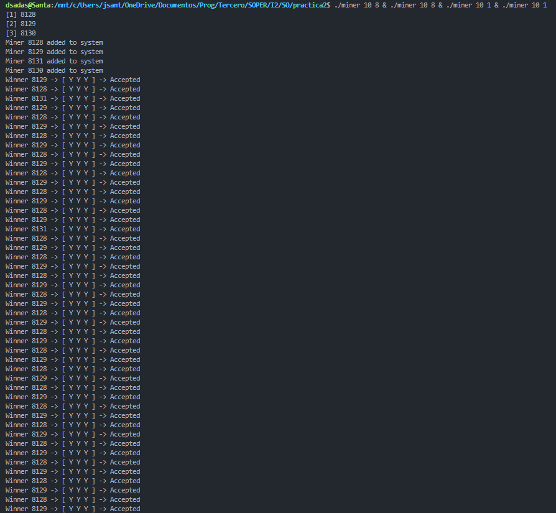
\includegraphics[width=1\textwidth]{image1.png}
    \caption{Ejecución de 4 mineros simultáneos durante 10 segundos. Se lanzaron dos procesos con 8 hilos y dos procesos con 1 hilo.
     Como se observa en las líneas de `Winner', los PIDs correspondientes a los procesos con 8 hilos acaparan la inmensa mayoría de 
     las victorias en las rondas, demostrando que un mayor número de hilos permite explorar el espacio de hashes (\textit{Proof of Work}) de
      forma mucho más rápida y eficiente, ganando la condición de carrera por el semáforo \texttt{sem\_winner}.}
\end{figure}

\begin{figure}[H]
    \centering
    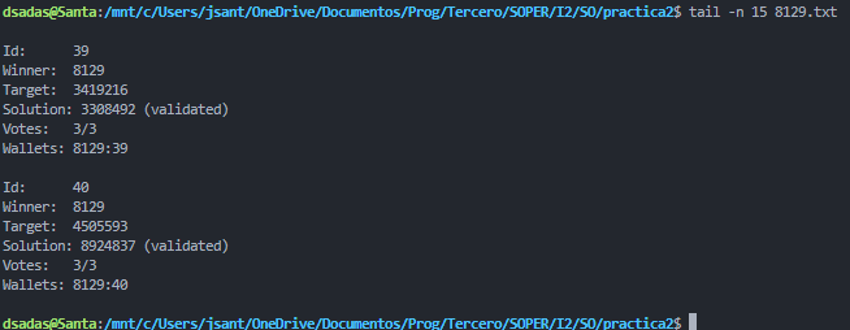
\includegraphics[width=1\textwidth]{image3.png}
    \caption{Registro de victorias generado por el proceso 8129. Como se puede observar, el minero ha registrado correctamente 
    el `Target' y la `Solution' de cada ronda, contabilizando los votos a favor (Y) de los demás procesos. El campo 'Wallets' 
    demuestra que el incremento de monedas locales se gestiona de forma segura tras la validación de la red.}
\end{figure}

\begin{figure}[H]
    \centering
    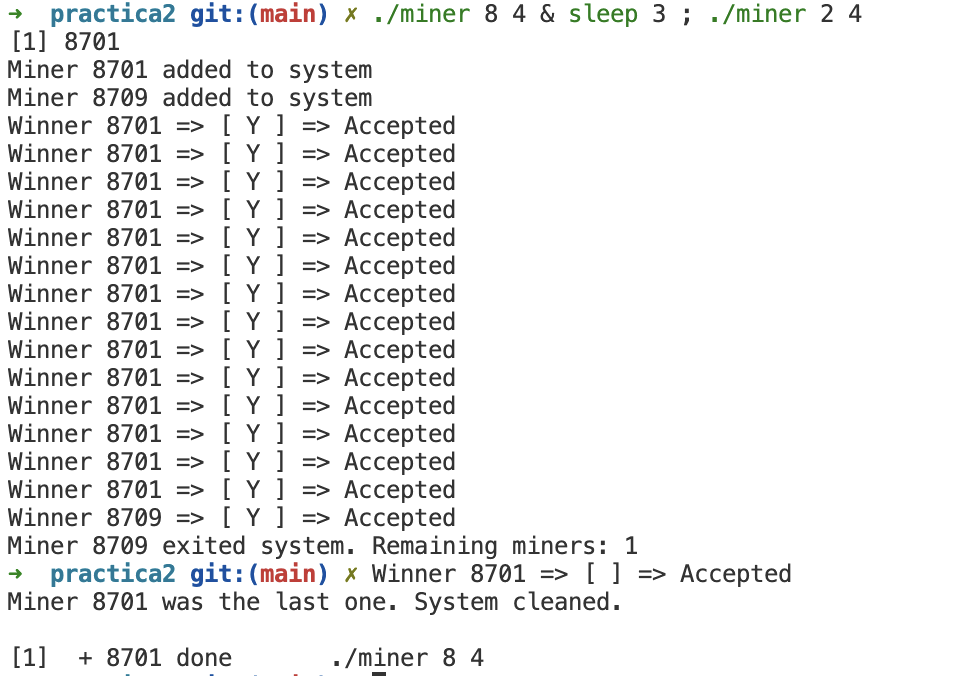
\includegraphics[width=1\textwidth]{image4.png}
    \caption{La ejecución demuestra que el sistema es totalmente robusto y no sufre \textit{deadlocks}: 
    Ambos procesos se registran correctamente y logran votar de forma concurrente (\texttt{[ Y ] -> Accepted}). 
    Cuando el minero de 2 segundos agota su alarma, sale de forma ordenada, actualiza el contador de procesos restantes y 
    libera sus recursos sin interrumpir al otro. El minero de 8 segundos detecta inmediatamente que se ha quedado solo. 
    Cumpliendo con los requisitos, el sistema entra en espera pasiva sin consumir recursos de forma innecesaria hasta que se 
    agota su tiempo y limpia el sistema.
     Al expirar el tiempo del último minero, este detecta que es el único que queda en el sistema y se encarga de ejecutar los \texttt{sem\_unlink} y 
     eliminar los ficheros \texttt{.tgt}, \texttt{.pid} y \texttt{.txt}, dejando el entorno completamente limpio (System cleaned) y evitando fugas de memoria en el sistema operativo.}
\end{figure}

\subsection{Pruebas con valgrind}
Para garantizar la robustez del sistema, se analizó el código utilizando Valgrind (se puede ejecutar con \texttt{make valgrind}). 
Los resultados confirmaron que no existen fugas de memoria tras la limpieza del último minero.
\begin{figure}[H]
    \centering
    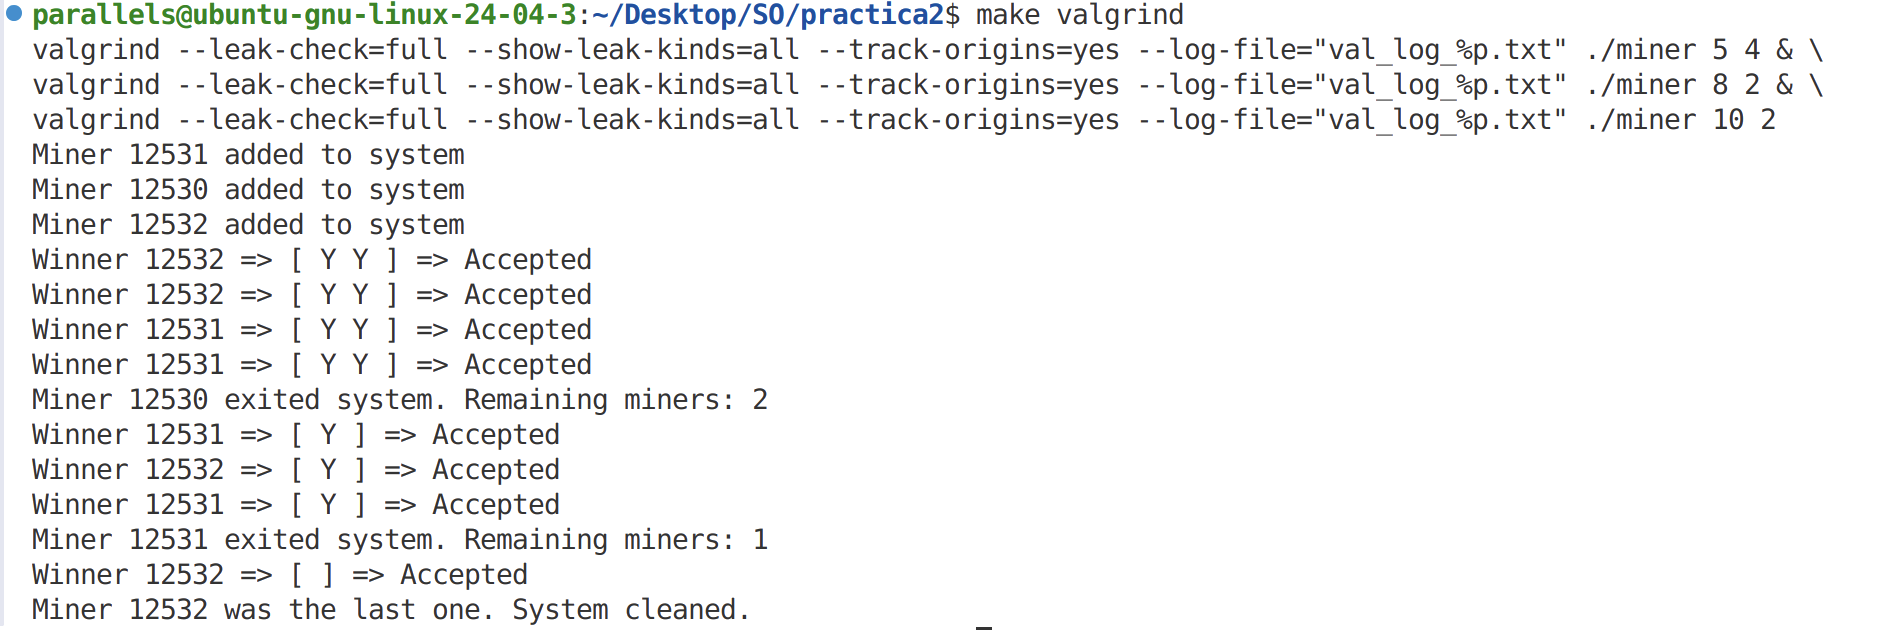
\includegraphics[width=1\textwidth]{image5.png}
    \caption{En la captura, muestra la ejecución del programa con valgrind, donde las salidas de valgrind se ha redireccionado a ficheros}.
\end{figure}
\begin{figure}[H]
    \centering
    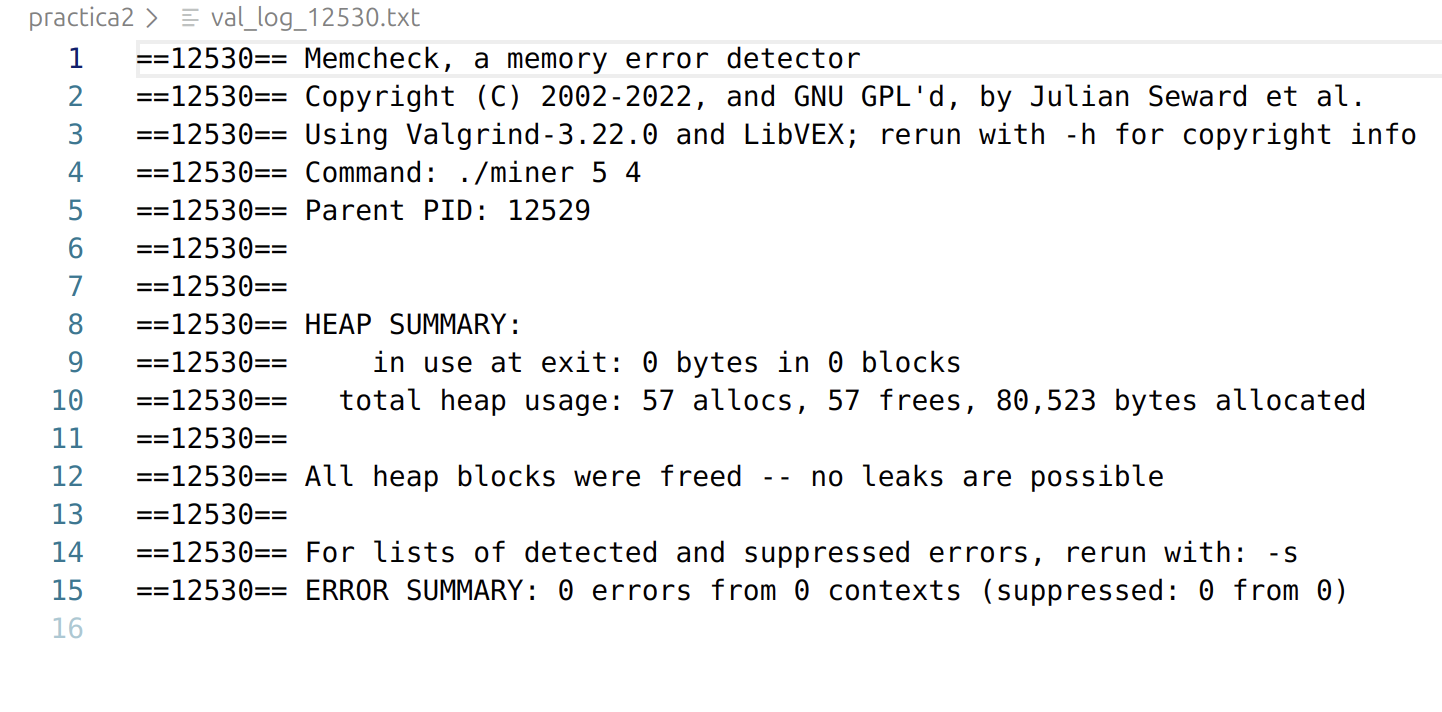
\includegraphics[width=1\textwidth]{image6.png}
    \caption{Ejemplo de salida de valgrind, donde podemos ver que no hay problema de fuga de memoria}.
\end{figure}
\section{Conclusión y Respuesta a las cuestiones del enunciado}
\begin{description}
    \item[Pregunta a:] \textbf{¿Se produce algún problema de concurrencia en el sistema descrito?} \hfill \\
    Sí, el sistema tiene varios puntos donde la concurrencia puede causar fallos. 
    El problema principal es el acceso a los ficheros compartidos como \texttt{pids.pid}, \texttt{target.tgt} y \texttt{vote.txt}, 
    ya que al ser procesos independientes, varios podrían intentar escribir o leer a la vez, corrompiendo los datos. También hay un problema de 
    ``condición de carrera'' al final de cada ronda: varios mineros pueden encontrar una solución válida casi al mismo tiempo y ambos intentarían 
    proclamarse ganadores simultáneamente.
    
    \item[Pregunta b:] \textbf{¿Cómo se ha solucionado en el planteamiento dado?} \hfill \\
    La solución se basa en el uso de semáforos con nombre de POSIX que actúan como mutex para garantizar la exclusión mutua. 
    Cada vez que un proceso necesita acceder a un fichero, debe adquirir el semáforo correspondiente (\texttt{sem\_pid}, \texttt{sem\_target}, 
    \texttt{sem\_votes}). Para la competición por la victoria, se utiliza el semáforo \texttt{sem\_winner} con la función \texttt{sem\_trywait}, 
    lo que asegura que solo el primer minero en realizar la llamada se convierta en el ganador oficial. Asimismo, se implementó un bloqueo de señales y el uso de \texttt{sigsuspend}
     para evitar la pérdida de notificaciones críticas durante la ejecución de estas secciones.

    \item[Pregunta c:] \textbf{¿Es sencillo, o siquiera factible, organizar un sistema de este tipo usando únicamente señales?} \hfill \\
    No es nada sencillo y, en la práctica, no es factible para un sistema así. Las señales son solo avisos; no pueden enviar datos 
    como la solución del hash o los votos de cada minero. Además, las señales no sirven para bloquear el acceso a un archivo; si usáramos solo señales,
     no tendríamos forma de garantizar que dos procesos no escriban en el mismo fichero a la vez, lo que acabaría rompiendo toda la lógica de la cadena.

    \item[Pregunta d:] \textbf{¿Cuáles son los mineros que tienden a ganar más monedas?} \hfill \\
    Como se puede ver en las pruebas de rendimiento (ver la Figura 2), los mineros que más ganan son los que tienen más hilos (\texttt{N\_THREADS}). 
    Al tener más hilos, el proceso divide el trabajo de búsqueda y puede probar muchos más hashes por segundo en paralelo. En la captura de la Figura 2, 
    se ve claramente que los procesos 8128 y 8129 (lanzados con 8 hilos) ganan casi todas las rondas, mientras que los de 1 hilo (8130 y 8131) casi nunca 
    llegan a tiempo de encontrar la solución.
\end{description}
\end{document}